\documentclass[12pt]{article}
\usepackage[usenames]{color} %used for font color
\usepackage{amsmath, amssymb, amsthm}
\usepackage{wasysym}
\usepackage[utf8]{inputenc} %useful to type directly diacritic characters
\usepackage{graphicx}
\usepackage{caption}
\usepackage{subcaption}
\usepackage{float}
\usepackage{mathtools}
\usepackage [english]{babel}
\usepackage [autostyle, english = american]{csquotes}
\MakeOuterQuote{"}
\graphicspath{ {./} }
\newcommand{\Z}{\mathbb{Z}}
\newcommand{\N}{\mathbb{N}}
\newcommand{\R}{\mathbb{R}}
\newcommand{\Q}{\mathbb{Q}}
\newcommand{\prob}{\mathbb{P}}
\newcommand{\degrees}{^{\circ}}
\DeclarePairedDelimiter\ceil{\lceil}{\rceil}
\DeclarePairedDelimiter\floor{\lfloor}{\rfloor}

\author{Tianshuang (Ethan) Qiu}
\begin{document}
\title{Math 74, Week 6}
\maketitle

\section{Mon Lec, 1a}
Base case: $n=1, n=2, a_1=3, a_2=5$, base cases hold.
\newline
Assume that for some $n \in \N$, all $m \in \N 1, 1 \leq m \leq n$ satisfies this identity, we have
$$a_{n+1}=3a_n-2a_{n-1}=3(2^n+1)-2(2^{n-1}+1)=3\times 2^n+3-2\times 2^{n-1}-2$$
$$=2^{n-1}(6-2)+1=2^{n-1}(2^2)+1=2^{n+1}+1$$
Thus we have proven the inductive case. Q.E.D.

\section{Mon Lec, 3c}
Lemma: a sequence given by $f_n=1/\sqrt5 (\phi^{n} - \bar \phi^{n})$ where $\phi = (1+\sqrt5)/2, \bar \phi = (1-\sqrt5)/2$ has the property $f_n+f_n+1 = f_n+2$ for $n \geq 0$
\newline
Base case: $n = 0$, $f_0 = 0, f_1=1, f_2=1$, base case holds.
Assume that for some $n$, the statement hodls for all $m\leq n$.
\newline
Consider $f_{n+1}$, $$f_n = \frac{1}{\sqrt5}((\frac{1+\sqrt5}{2})^n-(\frac{1-\sqrt5}{2})^n)$$
We get use this property to get a similar result for $f_{n-1}$. Now we add them together:
$$f_n+f_{n-1}=\frac{1}{\sqrt5}((\frac{1+\sqrt5}{2})^n-(\frac{1-\sqrt5}{2})^n+(\frac{1+\sqrt5}{2})^{n-1}-(\frac{1-\sqrt5}{2})^{n-1})$$
$$=\frac{1}{\sqrt5}(((\frac{1+\sqrt5}{2})^{n-1}(3+\sqrt5)/2)-(\frac{1-\sqrt5}{2})^{n-1}(3+\sqrt5)/2)$$
Since $(3+\sqrt5)=(1+\sqrt5)^2/2$, the expression simplifies to
$$=\frac{1}{\sqrt5}((\frac{1+\sqrt5}{2})^{n+1}-(\frac{1-\sqrt5}{2})^{n+1})$$.
Thus we have proven the fibbonacci property from the closed form.
\newline
Base case: $n=0, m=0, f_n=1, f_m=1, f_{n+m+1}=2$, base case holds.
\newline
For any $n, m \in \N$, assume that the statement is true for all $n'\leq n, m' \leq m$. Now consider $n+1$ and $f_{n+m+2}$.
\newline
Using our inductive hypothesis, we know that $f_{n+m+1}=f_mf_n + f_{m+1}f_{n+1}$
\newline
Now consider $f_mf_{n+1}+f_{m+1}f_{n+2}$, use our lemma to get that it is equal to $f_m(f_n+f_{n-1})+f_{m+1}(f_n+f_{n+1})$
$$=f_mf_n+f_mf_{n-1}+f_{m+1}f_n+f_{m+1}f_{n+1}$$
Now we apply IH,
$$=f_{m+n}+f_{m+n+1}=f_{m+n+2}$$
The last step is using our lemma (the fibbonacci identity). Thus we have proven the inductive step. Q.E.D.

\section{Mon Lec, 4a}
\begin{figure}[h]
    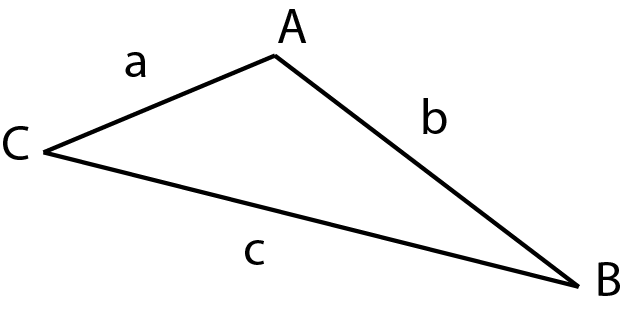
\includegraphics[width = 100mm]{GRAPH1.png}
\end{figure}
Base case: let there be three people, they form a triangle. Let the sides have length $a<b<c$. We can see that A and C will exchange pies, and B will throw at A, leaving him the survivor. Therefore base case holds.
\newline
Assume that for some odd $n$, the statement holds for all odd $m \leq n$. Now consider $n+2$.
\newline
We first remove the two people who are closest to each other. We call this the alternate game. Then the remaining $n$ people satisfies the inductive hypothesis, and there will be one survivor. Now consider the original game, since these two removed people are closest to each other, they will throw the pie at each other.
\newline
Then we break down the remaining players into two scenarios when we add the two back: the two new players are closer than their original targets, or they are further than their original targets.
\newline
In either case they will not throw their pies at the survivor in the alternate game. Therefore he will still be the survivor in the original game.
\newline
Thus we have proven the inductive case. Q.E.D.
\newpage

\section{Mon Dis, 4}
Base case: $n = 1, S = \{1,2\}, 1 \mid 2$, base case holds.
\newline
Assume that for $n \in \N$, the statement holds for $m \leq n$. Consdier $n+1$ and a set $S = \{a_1, a_2, ..., a_{n+2}\}$. We break it down into two cases.
\paragraph{If $a_{n+1}\leq 2n$}
Then we can simply take $S' = S \setminus a_{n+2}$, now we have a set that has $n+1$ elements, and the largest one is less than $2n$, so we can apply the inductive hypothesis and conclude that there is an integer that divides another in $S'$.
\paragraph{If $a_{n+1}> 2n$}
Now if $a_{n+1}>2n$, and the maximum of the set cannot exceed $2n+22$, we must have $a_{n+1}=2n+1. a_{n+2}=2n+2$. Now if $(n+1)\in S$, we will have $n+1 \mid 2n+2$. Otherwise, take the set $\{a_1, a_2, ..., a_n, n+1\}$, all of these are less than $2n$ since we know what $a_{n+1}$ and $a_{n+2}$ are. Now we can apply the inductive hypothesis to this set since it has $n+1$ items. Therefore there must be two integers that divides each other.
\newline
Thus we have proven the inductive case. Q.E.D.

\section{Mon Dis, 7}
Base case: $n=1$, we can simply take a block out, the remaining 3 form an $L$ shape. Base case holds
\newline
Assume that for some $n \in \N$, the statement holds for all $m \leq n$, now consider $2^{n+1} \times 2^{n+1}$. We first divide the square into four squares of $2^n \times 2^n$. Take the right most square and remove a single tile. By the inductive hypothesis this square is tilable with $L$'s since it has $2^n \times 2^n$ tiles. Now for the remaing three squares, we remove one tile at the center like this:
\newline
\begin{figure}[H]
    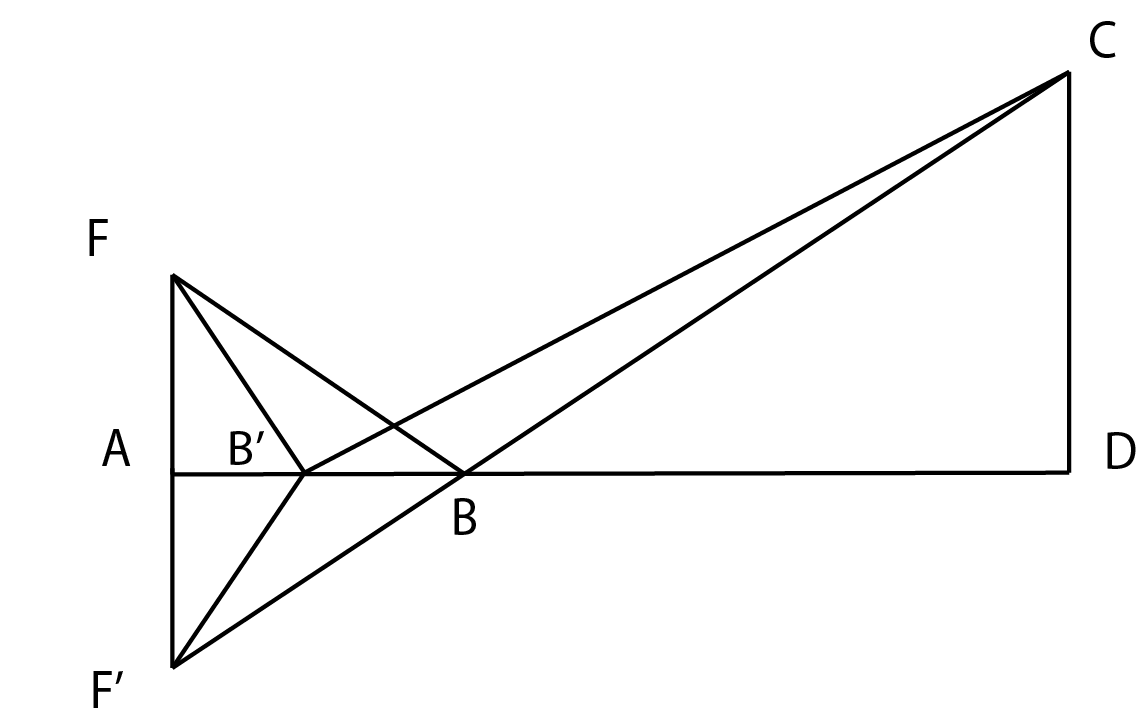
\includegraphics[width = 100mm]{GRAPH2.png}
\end{figure}
Now the remaining 3 tiles can be filled with a single $L$. Thus we have proven the inductive step. Q.E.D.

\newpage

\section{Wed Lec, 5}
Let our 9 digit number be represented by $abcde2021$. Using the subtraction theorem we know that $abcde0000/2021$ must be an integer.
\newline
We can factor $2021 = 43 \times 47$, so it shares no factors with 10000. So $2021 \mid abcde$. Now the amount that we are seeking is equal to the amount of 5 digit numbers that is divisible by 2021
$$\floor*{\frac{99999}{2021}}-\floor*{\frac{9999}{2021}} = 49-4=45$$
\newpage

\section{Wed Dis, 6}
$$(y-\frac{1}{y})^3 = x^3$$
$$y^3 -3 \frac{1}{y} + 3 y-\frac{1}{y^3} = x^3$$
$$y^3-\frac{1}{y^3}+3(y-\frac{1}{y})=x^3$$
$$y^3-\frac{1}{y^3}+3x = x^3$$
$$y^3-\frac{1}{y^3}= x^3-3x$$
\newpage

\section{Fri Lec, 3b}
Since $a \equiv b \bmod 6$, we have $a = 6n + k$, $b = 6m + k$, where $m,n,k \in \Z$.
\newline
Let $h \in \Z$, we multiply $a, b$ by $h$: $ah = 6nh + kh$, $bh = 6mh + kh$.
\newline
Since mutiples of 6 will always be equivalent to 0 when modded by 6, the only things that are left on both sides are $kh$, and $kh \equiv kh \bmod 6$.
\newline
Q.E.D.

\section{Fri Lec, 7}
We factor 12 into $3 \times 2^2$, and 15 into $3 \times 5$. Since our perfect square needs to have these as factors, $xy^2$ must have 3 as a factor, and $xy$ must have 5 as a factor.
\newline
Furthermore, since $xy$ has 5 as a factor, $xy^2$ must have 25 as a factor since the $12xy^2$ is a perfect square and 12 cannot be divided by 5. Now we attempt to construct one such number. let $y = 5$, $x=3$, $12xy^2 = 900 = 30^2, 15xy = 225 = 15^2$. $x+y = 8$

\end{document}
